
\noindent We are on our way to building a conformal quantum field theory (CQFT). So far, we have analyzed the consequences of conformal symmetries on the observables of a quantum field theory. \\

\noindent The observables of a quantum field theory, not necessarily self-adjoint as in quantum theory, are indirectly observable, as they are the correlation functions derivable from the direct observables of scattering amplitudes in scattering experiments. \\

\noindent We have found that the two-point correlation functions under the assumed constraints of a conformal field theory behave as

\begin{equation}
\langle \hat{\phi}_\alpha (x) \hat{\phi}_\beta (y) \rangle \sim \frac{1}{|x-y|^{d_\alpha + d_\beta}}.
\end{equation}

\noindent To actually construct a conformal quantum field theory (CQFT), we use the path integral approach as an efficient tool to (hopefully) yield proper, according to the theory at hand, quantum observables. In the path integral sppraoch, we have a ``box'' into which we put classical data, namely the action $S[\phi]$, a functional of the fields, and get wuantum data as output in the form of time-ordered correlation functions

\begin{equation}
\langle \mathcal{T} [ \hat{\phi} (x_1) \dots \hat{\phi} (x_n) ] \rangle \equiv \frac{\int \mathcal{D}\phi \, \phi (x_1) \dots \phi (x_n) e^{iS[\phi]}}{\int \mathcal{D} \phi \, e^{iS[\phi]}}.
\end{equation}

\noindent \textbf{Goal}: Our goal is to take a classical CFT and calculate the quantum generators of conformal symmetries corresponding to some CQFT. \\

\noindent \textbf{Note on imaginary time}: \\

\noindent We work with imaginary time $t \rightarrow -i \beta$ via analytic continuation, also called Wick rotation for two reasons.

\begin{enumerate}
\item It is convenient since things will converge better.
\item It makes direct contact with statistical physics.
\end{enumerate}

\noindent To the second point, Wick rotation of the time coordinate turns all formulae for a quantum system, eith unitary time evolution, into statements about partition functions and thermal systems at temperature $\beta$. In other words, Wick rotation maps the unitary generators of time translation to a non-unitary semigroup with fixed points being the ground state

\begin{equation}
U(t) = e^{-it\hat{H}} \rightarrow S(\beta) = e^{-\beta \hat{H}}.
\end{equation}

\noindent From $S(\beta)$, we simply take the trace and get the partition function, for a system in thermal equilibrium with a reservoir at inverse temperature $\beta$

\begin{equation}
Z = \text{tr} (S(\beta)) = \text{tr} (e^{-\beta \hat{H}}).
\end{equation}

\noindent This contact with statistical physics and thermal states of systems is also interesting because in studying phase transitions, at critical points, the symmetry group is enlarged, and the system exhibits, for example, dilation and scale invariance. Phase transitions are examples of conformal field theories, though with non-unitary representations of the symmetry group. See \textit{Cardy, Scaling \& Phase Transitions} for reference. \\

\noindent Since our goal is to construct unitary representations of the conformal group of Minkowski space, for the reasons above, we Wick rotate and work with imaginary time. After our calculations, we Wick rotate back into real time, as much as allowed by holomorphic functions. \\

\noindent The path integral, our tool for calculating quantum obervables, under Wick rotation $t \rightarrow -i \beta$ transforms as 

\begin{equation}
\int \mathcal{D} \phi \, e^{i S[\phi]} \rightarrow \int \mathcal{D} \phi \, e^{iS[\phi]}.
\end{equation}

\subsection*{Constructing a CQFT}

\noindent Suppose we have a tuple of classical fields $\phi(x)$, and let $S$ be the action of the fields with assumed invariance under infinitesimal conformal symmetry transformations (up to a total derivative).

\begin{equation}
\phi(x) \rightarrow \phi' (x) = \phi (x) - i \omega_a (x) G_a \phi (x)
\end{equation}

\noindent Where $G_a$ is a symmetry transformation matrix. For example,

\begin{align}
\text{Translations: }& G_a \simeq -i \partial_\nu \\
\text{Dilations: }& G_a \simeq -i x^\nu \partial_\nu - i \Delta_a.
\end{align}

\noindent Note that time-ordering of quantum field operators is implicit whenever the LHS is a correlator and the RHS is a path integral, and define 

\begin{equation}
\hat{X} \equiv \mathcal{T} [ \hat{\phi} (x_1) \dots \hat{\phi} (x_n) ].
\end{equation}

\noindent By the path integral prescription, the time-ordered quantum correlation function is given by classical (not time-ordered) data, after Wick rotation, as

\begin{equation}
\langle \hat{X} \rangle = \frac{1}{Z} \int \mathcal{D} \phi \, X e^{iS[\phi]} = \frac{1}{Z} \int \mathcal{D} \phi \, \phi (x_1) \dots \phi (x_n) e^{iS[\phi]}
\end{equation}

\noindent Where we have written the partition function $Z$, since we have Wick-rotated into imaginary time and

\begin{equation}
\int \mathcal{D} \phi \, e^{iS} \rightarrow \text{tr}(e^{-\beta H}) = Z.
\end{equation}

\noindent Under the infinitesimal transformation above, \textit{assume} that the measure is invariant, such that $\mathcal{D} \phi' = \mathcal{D} \phi$. Recall that the action is invariant up to a total derivative. Then the correlation function, including the product of time-ordered quantum field operators, becomes

\begin{equation}
\langle \hat{X} \rangle = \frac{1}{Z} \int \mathcal{D} \phi' \,\, (X + \delta X) e^{-S[\phi] - \int dx \, \partial_\mu j_a^\mu \omega_a (x)}
\end{equation}

\noindent Where $X' = X + \delta X$, and to order $\omega_a$

\begin{equation}
X' = (\phi (x_1) - i \omega_a G_a \phi (x_1)) (\phi (x_2) - i \omega_a G_a \phi (x_2)) \dots
\end{equation}

\noindent Which makes the infinitesimal change in $X$ to be

\begin{align}
\delta X &= -i \sum_{j=1}^n \, \left(\phi(x_1) \dots G_a \phi(x_j) \dots \phi(x_n) \right) \omega_a (x_j) \\
&= -i \int dx \,\, \omega_a (x) \sum_{j=1}^n  \, \left(\phi(x_1) \dots G_a \phi(x_j) \dots \phi(x_n) \right) \delta (x-x_j).
\end{align}

\noindent Insert this into the equation for $\langle \hat{X} \rangle$ and distribute to get

\begin{align}
\langle \hat{X} \rangle &= \frac{1}{Z} \int \mathcal{D} \phi \left( X e^{-S} + \delta X e^{-S} + X e^{-S}\left(\int dx \partial_\mu j_a^\mu \omega_a (x)\right) \right) \\
\langle \hat{X} \rangle &= \langle \hat{X} \rangle + \langle \delta \hat{X} \rangle - \int dx \, \partial_\mu \langle \hat{j}_a^\mu \hat{X} \rangle \omega_a (x) \\
0 &= \langle \delta \hat{X} \rangle - \int dx \, \partial_\mu \langle \hat{j}_a^\mu \hat{X} \rangle \omega_a (x).
\end{align}

\noindent By the infintesimal transformation and the invariance of the action, we have inserted the conserved classical current into the path integral presecription and have gotten a quantum operator in return! We find that the quantization of the infinitesimal change $\delta X$ is equal to the integral of the divergence of the quantization of the product $j_a^\mu X$. \\

\noindent From this equality, which holds for all $\omega_a (x)$, extract the local relation of how the quantum fields transform according to the transformation-generating conserved current. Pull off the integral by the insertion of the delta function into $\delta X$ above. The local equality, called the \textit{Ward identity} is then

\begin{equation}
\frac{\partial}{\partial x^\mu} \langle \hat{j}_a^\mu (x) \hat{\phi} (x_1) \dots \hat{\phi} (x_n) \rangle = -i \sum_{j=1}^n \, \delta (x-x_j) \langle\hat{\phi} (x_1) \dots G_a \hat{\phi} (x_j) \dots \hat{\phi} (x_n) \rangle
\end{equation}

\noindent The Ward identity is the principal tool by which we quantize symmetries and showing how the symmetries are implemented on quantum correlation functions. \\

\noindent Integrate the Ward identity over all of spacetime (assuming good decay), and show that the quantum correlation function is invariant under the infinitesimal symmetry transformation

\begin{equation}
\delta_\omega \langle \hat{\phi} (x_1) \dots \hat{\phi} (x_n) \rangle \equiv -i \omega_a (x) \sum_{j=1}^n \, \langle\hat{\phi} (x_1) \dots G_a \hat{\phi} (x_j) \dots \hat{\phi} (x_n) \rangle = 0.
\end{equation}

\noindent Recall that the conserved charge corresponding to the \textit{generator} of some symmetry is gotten by integrating the time component of the conserved current

\begin{equation}
\hat{Q}_a = \int d^{d_a} x \,\, \hat{j}_a^0 (x).
\end{equation}

\noindent Integrate the Ward identity now over a thin slice of time $t_- < t < t_+$, instead of the entire spacetime, and suppose that there is one point of time $x_1^0 = t$ that is contained within the slice, and all others are sufficiently far away.

\begin{figure}[H]
	\centering
	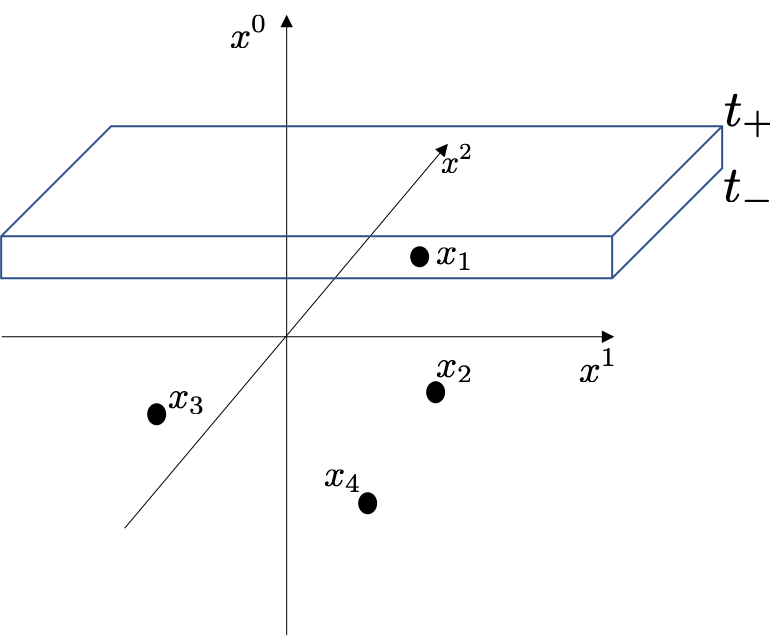
\includegraphics[width=2in]{images/ward_timeslice.png} 
\end{figure} 

\noindent The LHS of the Ward identity becomes 

\begin{equation}
\langle \hat{Q}_a (t_+) \hat{\phi} (x_1) \hat{Y} \rangle - \langle \hat{Q}_a (t_-) \hat{\phi} (x_1) \hat{Y} \rangle = -i \langle G_a \hat{\phi} (x_1) \hat{Y} \rangle
\end{equation}

\noindent Where $\hat{Y} = \hat{\phi} (x_2) \dots \hat{\phi} (x_n)$. \\

\noindent Let the inverse temperature go to infinity $\beta \rightarrow \infty$, such that we have the vacuum correlation function $\langle \hat{X} \rightarrow \bra{0} \hat{X} \ket{0}$. Suppose that there is a point of time ahead of the slice-contained point $x_j^0 > x_1^0$, and in the limit of an inifnitesimal time slice$t_- \rightarrow t_+$, the expression for the Ward identity above becomes

\begin{equation}
\bra{0} [ \hat{Q}_a, \hat{\phi} (x_1) ] \hat{Y} \ket{0} = -i \bra{0} G_a \hat{\phi} (x_1) \ket{0}.
\end{equation}

\noindent This is true for all $\hat{Y}$, such that we have the commutator bracket, starting with classical data, for conserved charges and quantum field operators that shows that passing the quantum conserved charge operator over the field is tantamount to applying the symmetry transformation $G_a$

\begin{equation}
[ \hat{Q}_a, \hat{\phi} ] = -i G_a \hat{\phi}.
\end{equation}

\noindent For example, translations transform the field as $\phi' (x) = \phi (x) - \epsilon^\mu \partial_\mu \phi (x)$ with symmetry transformation matrix $G_a = i \partial_\mu$, and the conserved charge operator is the total momentum operator $\hat{Q}_\mu \equiv \hat{P}_\mu$. \\

\subsection*{Ward Identities for Conformal Symmetries}

\noindent Let $\hat{X}$ be the product of local quantum field operators as before, and consider the invariants of conformal symmetry transformations. The conserved current is the \textit{energy-momentum tensor} $\hat{T}^\mu_\nu$, where we assume that $T_\mu^\nu$ (classical) is traceless $T^\mu_\mu = 0$ and symmetric $T_{\mu\nu} = T_{\nu\mu}$, which does not necessarily hold quantumly. \\

\noindent \textbf{Translation}: \\

\begin{equation}
\partial_\mu \langle \hat{T}^\mu_\nu \hat{X} \rangle = -i \sum_j \delta(x-x_j) \partial_{x_j^\nu} \langle \hat{X} \rangle.
\end{equation}

\noindent \textbf{Rotation}: \\

\begin{equation}
\langle (\hat{T}^{\rho\nu} - \hat{T}^{\nu\rho} ) \hat{X} \rangle = -i \sum_j \delta(x-x_j) s_j^{\nu\rho} \langle \hat{X} \rangle
\end{equation}

\noindent Since $j^{\mu\nu\rho} = T^{\mu\nu} x^\rho - T^{\mu\rho} x^\nu$ (\textbf{Exercise}). Note that $s_j^{\nu\rho}$ is the spin matrix representation of the $j^{th}$ field vector, and is equal to one for spinless particles. \\

\noindent \textbf{Dilation}: \\

\begin{equation}
\langle \hat{T}^\mu_\mu \hat{X} \rangle = - \sum_j \delta(x-x_j) \Delta_j \langle \hat{X} \rangle.
\end{equation}

\noindent Since $G \equiv D = -i x^\nu \partial_\nu - i \Delta$ (\textbf{Exercise}). \\ \\

\noindent Next, we work out the two-dimensional case and rewrite the Ward identities in complex coordinates. We will then work out examples of energy-momentum tensors for free bosons, and see that the remaining degrees of freedom of the energy-momentum tensor for the \textit{Virasoro algebra}.